\chapter{Methods, Class Variables, and Instance Variables}

\section{Introduction: Real-Life Hook}

In a school, all students follow the same:
\begin{itemize}
    \item School name
    \item School rules
\end{itemize}

But each student has their own:
\begin{itemize}
    \item Name
    \item Roll number
    \item Marks
\end{itemize}

In programming:
\begin{itemize}
    \item \textbf{Class variables} are shared by everyone
    \item \textbf{Instance variables} are personal to each object
\end{itemize}

This chapter explains:
\begin{itemize}
    \item Methods
    \item Class variables
    \item Instance variables
    \item Their differences
\end{itemize}

\section{Concept: Methods in a Class}

\begin{definition}{Method}
A method is a \textbf{function defined inside a class} that describes the behavior of an object.
\end{definition}

Example:
\begin{verbatim}
class Student:
    def study(self):
        print("Student is studying")
\end{verbatim}

Methods:
\begin{itemize}
    \item Always have \texttt{self} as the first parameter
    \item Work on object data
\end{itemize}

\section{Instance Variables}

\begin{definition}{Instance Variable}
Instance variables store \textbf{data unique to each object}.
\end{definition}

Example:
\begin{verbatim}
class Student:
    def __init__(self, name):
        self.name = name
\end{verbatim}

Each object gets its own value:
\begin{verbatim}
s1 = Student("Ayesha")
s2 = Student("Rafi")
\end{verbatim}

\section{Class Variables}

\begin{definition}{Class Variable}
A class variable is a \textbf{variable shared by all objects of the class}.
\end{definition}

Example:
\begin{verbatim}
class Student:
    school_name = "Green Valley School"

    def __init__(self, name):
        self.name = name
\end{verbatim}

\begin{verbatim}
print(Student.school_name)
\end{verbatim}

\section{Accessing Variables}

\subsection{Accessing Instance Variables}

\begin{verbatim}
print(s1.name)
\end{verbatim}

\subsection{Accessing Class Variables}

\begin{verbatim}
print(Student.school_name)
\end{verbatim}

\section{Methods Using Both Variables}

\begin{verbatim}
class Student:
    school_name = "Green Valley School"

    def __init__(self, name, marks):
        self.name = name
        self.marks = marks

    def display(self):
        print("Name:", self.name)
        print("School:", Student.school_name)
        print("Marks:", self.marks)
\end{verbatim}

\section{Mini-Project: School Report System}

\textbf{Goal:} Use both class and instance variables.

\begin{verbatim}
class Student:
    school_name = "Sunrise High School"

    def __init__(self, name, marks):
        self.name = name
        self.marks = marks

    def report(self):
        print("School:", Student.school_name)
        print("Student:", self.name)
        print("Marks:", self.marks)

s1 = Student("Ayesha", 85)
s2 = Student("Rafi", 62)

s1.report()
s2.report()
\end{verbatim}

\section{Diagram: Class vs Instance Variables}

\begin{center}
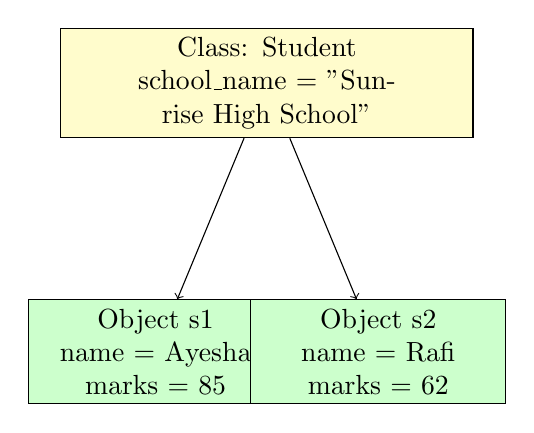
\begin{tikzpicture}[node distance=2cm]
\node (class) [draw, rectangle, fill=yellow!20, text width=5cm, align=center] {Class: Student\\
school\_name = "Sunrise High School"};
\node (obj1) [draw, rectangle, fill=green!20, below left of=class, yshift=-2cm, text width=3cm, align=center] {Object s1\\
name = Ayesha\\
marks = 85};
\node (obj2) [draw, rectangle, fill=green!20, below right of=class, yshift=-2cm, text width=3cm, align=center] {Object s2\\
name = Rafi\\
marks = 62};

\draw[->] (class) -- (obj1);
\draw[->] (class) -- (obj2);
\end{tikzpicture}
\end{center}

\section{Difference Between Class and Instance Variables}

\begin{center}
\begin{tabular}{|l|l|l|}
\hline
\textbf{Feature} & \textbf{Class Variable} & \textbf{Instance Variable} \\
\hline
Belongs to & Class & Object \\
Shared & Yes & No \\
Accessed by & Class name & Object name \\
Memory & One copy & Multiple copies \\
\hline
\end{tabular}
\end{center}

\section{Common Beginner Mistakes}

\begin{itemize}
    \item Using instance variables instead of class variables
    \item Changing class variables through objects
    \item Forgetting \texttt{self} in methods
\end{itemize}

\section{Key Concepts}

\begin{itemize}
    \item Methods define behavior
    \item Instance variables store object-specific data
    \item Class variables are shared by all objects
    \item Proper use improves program design
\end{itemize}

\section{End-of-Chapter Exercises}

\subsection{Very Short Questions}

\begin{enumerate}
    \item What is a method?
    \item What is a class variable?
    \item Which variable type is shared by all objects?
\end{enumerate}

\subsection{Short Answer Questions}

\begin{enumerate}
    \item Explain the difference between class and instance variables.
    \item Write a class with one class variable and one instance variable.
    \item Why should class variables be accessed using the class name?
\end{enumerate}

\subsection{Activity-Based Exercises}

\begin{enumerate}
    \item Create a \texttt{LibraryBook} class with a shared library name.
    \item Build a \texttt{Employee} class with company name as class variable.
    \item Modify the Student class to count total students using a class variable.
\end{enumerate}

\section{Teacher Notes}

\marginnote{
\textbf{Learning Objectives}
\begin{itemize}
    \item Students understand methods clearly
    \item Students can distinguish class and instance variables
    \item Students apply correct variable usage
\end{itemize}

\textbf{Teaching Tips}
\begin{itemize}
    \item Use school examples for class variables
    \item Draw memory diagrams on the board
    \item Encourage students to explain code in words
\end{itemize}

\textbf{Assessment}
\begin{itemize}
    \item Correct variable classification
    \item Clean object-oriented design
\end{itemize}
}